

\section{Experiments and Analysis}

This Section reports the experiments performed to validate our model.
First, we will introduce the ChaLearn dataset, and then present the experimental protocol we followed.
In Section~\ref{sec:results}, we will present and analyse the obtained results, including a discussion
on the modeling elements.
Finally, Section~\ref{sec:ComputationalComplexity} will briefly discuss the computational complexity of the approach.



\subsection{Chalearn LAP Dataset}
\label{sec:chalearn}

\mycomline{In this part, provide more information about the dataset: description, content, types of gestures (what are the classes), illustration of the gestures with some pictures (esp. for gestures that have impact on data -for example, expand fig 14 where yoou have the two ok and noncepiu examples with other ones, and put it earlier in the document. why is the dataset challenging ?\\
Also, provide some statistics about the dataset:
 rough duration of the gestures (average, min max). How many person are performing the gestures, how many occurrences per class, is the dataset balanced}

The dataset used in this work is provided by the ChaLearn LAP \cite{chalearnLAP} gesture spotting challenge\footnote{\href{http://gesture.chalearn.org/homewebsourcereferrals}{http://gesture.chalearn.org/homewebsourcereferrals}}.
%
It contains 940 videos sequences, each performed by a single person (X persons are involved in the dataset)
and composed of 10 to 20 gesture instances for a total of $14\,000$ gestures.
%
There are 20 gesture classes,
\mycomline{(to be presented/commented)}

In terms of data, three modalities are provided with the input videos: the sequence of skeleton joints, and the RGB and depth images
(including a segmentation of the person performing the gesture).
%For the input sequences, there are three modalities provided, \emph{i.e.} skeleton, RGB and depth images (with user segmentation).
% This dataset  is on ``multiple instance, user independent learning and continuous gesture spotting"~\cite{ICMI} of gestures.
% In the 3 track, there are more than 14,000 gestures.




\subsection{Experimental protocol}

\subsubsection{Training and evaluation protocol.}

We follow the ChaLearn experimental protocol, in which the input sequences are split into 700 videos for training, and 240 sequences for testing and reporting results.
Note that the   test sequences  are not segmented a priori and the gestures must be detected within a continuous data stream
which, in addition to the targeted gestures, also contains noisy and out-of-vocabulary gestures.
%
Furthermore, in the experiments, we split the training videos into 650 videos for learning the actual neural network model parameters, and 50 videos
used as validation data for monitoring the training performance or selecting hyper-parameters.


\subsubsection{Performance measures.}

Several measures can be used to evaluate the gesture recognition performance.
%
In this work, we adopted the ChaLearn performance measure known as the Jaccard index, which relies on a frame-by-frame prediction accuracy.
More precisely, if $GT_i$ denotes the sequence of ground truth labels in video $i$, and $R_i$ the algorithm output, the Jaccard index
of the video is defined as:
\begin{equation}
\jaccardindex_i(GT_i, R_i) = \frac{N_s(GT_i, R_i)}{N_u(GT_i, R_i)}
\end{equation}
where $N_s(GT_i, R_i)$ denotes the number of frames where the ground truth and result agree on a gesture class,
and $N_u(GT_i, R_i)$ denotes the number of frames labeled as a gesture frame by  either the ground truth or the algorithm\footnote{Note that 'non gesture'
frames are thus excluded from the counts.}. The average of the $\jaccardindex_i$ over all test videos is reported as performance measure.
%
Note that experimentally, this measure tends to favours having more false positives than missing true positives, in order to increase the numerator.
%Effective ways to detect false positives should be an interesting aspect of future work.

Being defined at the frame level, the Jaccard index can vary due to variations of the segmentation (both in the ground truth and recognition)
at gesture boundaries, which can be irrelevant from an application viewpoint.
%
Thus, we also defined performance at the gesture event level by following the commonly used PASCAL challenge intersection over union criterion.
More precisely, if for a gesture segment $G$, we have $\frac{G \cap R}{G \cup R} >  0.5$, where R denotes a recognized gesture
segment of the same class, then the  gesture is said to be recognized.
%
If the same relation holds but with a gesture segment of another class, the prediction is incorrect.
Otherwise the gesture is rated as undetected. This allows us to define the $Recognized$, $Confusion$ and $Missed$ performance measures at the video level,
which are further averaged over test sequences for reporting.


\begin{figure*}[t]
        \centering
        \begin{subfigure}[c]{.8\textwidth}
                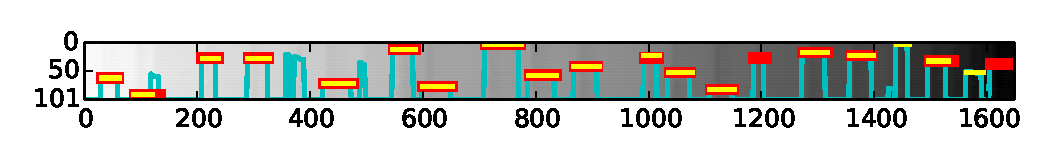
\includegraphics[width=\textwidth]{images/path/Sample0700_sk}
\vspace*{-3mm}
                \caption{Sample \#700 skeleton input path.}
                \label{Sample0700_sk}
        \end{subfigure}%
        ~ %add desired spacing between images, e. g. ~, \quad, \qquad, \hfill etc.
          %(or a blank line to force the subfigure onto a new line)

        \begin{subfigure}[c]{0.8\textwidth}
                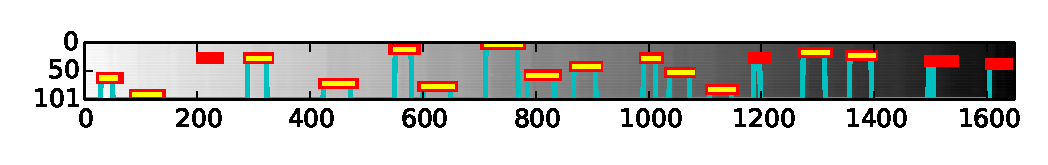
\includegraphics[width=\textwidth]{images/path/Sample0700_cnn}
\vspace*{-3mm}
                \caption{Sample \#700 depth and RGB input path.}
                \label{Sample0700_cnn}
        \end{subfigure}

        ~ %add desired spacing between images, e. g. ~, \quad, \qquad, \hfill etc.
          %(or a blank line to force the subfigure onto a new line)
        \begin{subfigure}[c]{0.8\textwidth}
                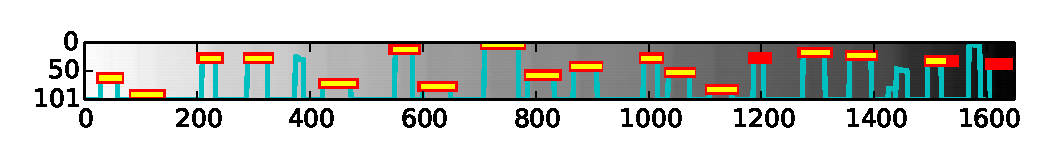
\includegraphics[width=\textwidth]{images/path/Sample0700_combined}
\vspace*{-3mm}
                \caption{Sample \#700 combined input path.}
                \label{Sample0700_combined}
        \end{subfigure}

  \caption{Viterbi decoding of the two modules and their fusion of sample sequence \#700. Top to bottom: skeleton, RGBD, multimodal fusion with x-axis representing the time and y-axis representing the hidden states of all the classes with the ergodic state at the bottom. Red lines are the ground truth labels, cyan lines represent the viterbi shortest path and yellow lines are the predicted labels. There are some complementary information of the two modules and generally the skeletal module outperforms the depth module. The fusion of the two could exploit the uncertainty, \emph{e.g.} around frame 200 the skeleton can help with the false negative predictions given by the 3DCNN module. Around frame 1450, the 3DCNN module can help suppress the false positive prediction given by skeleton module.
  }\label{Sample0700_comparison}
\end{figure*}

\subsubsection{Tested systems.}

We evaluated the recognition performance made by the HMM applied to the emission probabilities estimated from either
the skeleton data, the RGBD image data, the late fusion scheme, and the early fusion scheme.
%
Note that the HMM output was further filtered as follows to avoid false alarms.
First, predicted gesture segments of less than 20 frames were considered as noise and discarded.
%
In addition, longer but noisy gesture segments whose log-probability (including both emission and transition probabilities)  measured over the viterbi path
was lower than a threshold were discarded.
%
This threshold was set by optimizing the Jaccard index on the validation set  of the training data.


\subsection{Results}

The individual module results and the fusion results are shown in Tab. \ref{Table_score_fusion}. Note that the skeleton module generally performs better than the depth module, one reason could be that the skeleton joints learnt from~\cite{shotton2011real} lie in success of utilising huge and highly varied training data: from both realistic and synthetic depth images, a total number of 1 million images were used to train the deep randomised decision forest classifier in order to avoid overfitting. Hence, skeleton data is more robust.

From the frame based prediction, we also evaluate the gesture token classification rate using the commonly-used PASCAL overlap criterion: if the gesture is predicted correctly with more than 50\% overlap with the ground truth label, then the prediction is counted as a true positive. The results of the two individual modules and the score of the fused modules are shown in Tab.~\ref{Prediction}. From the confusion matrices in Fig.~\ref{confusion_matrix} we can observe the complimentary information between the skeleton input and the RGBD input.
% with the confusion matrices shown in Fig.~\ref{confusion_matrix}.
While many of the gestures in this data set could be mainly differentiated by examining the positions and motions of large joints such as the elbows and wrists,  some gestures differ primarily  in hand pose, \emph{e.g.} Fig. \ref{hand_differ}.
% From the confusion matrices in Fig.~\ref{confusion_matrix} we can observe the complimentary information between the skeleton input and the depth \& RGB input.
%%%%%%%%%%%%%%%%%%%%%%%%%%%%%%%%%%%%%%%%%%%%%%%%%%%%%%%%%%
%%%%%%%%%%%%%%%%%%%%%%%%%%%%%%%%%%%%%%%%%%%%%%%%%%%%%%%%%%
 \begin{table}[t]
   \centering
        \begin{tabular}{|l||*{2}{c|}}\hline
            {Module}
            &\makebox[5em]{Validation}&\makebox[5em]{Test}
            \\\hline\hline
            {\small Skeleton -- DBDN }            &  0.78266    & 0.77920 \\\hline
            {\small RGBD -- 3DCNN }      &  0.75163    & 0.71678 \\\hline%\hline
            {\small Multimodal Late Fusion }              &  0.81744    & 0.80910 \\\hline
            {\small Multimodal Early Fusion }             &  0.80014    & 0.79800 \\\hline
        \end{tabular}

    \caption{
    Comparison of results in terms of Jaccard index between different network structures and various modules.
          }
          \label{Table_score_fusion}
\end{table}
%%%%%%%%%%%%%%%%%%%%%%%%%%%%%%%%%%%%%%%%%%%%%%%%%%%%%%%%%%


%%%%%%%%%%%%%%%%%%%%%%%%%%%%%%%%%%%%%%%%%%%%%%%%%%%%%%%%%%

 \begin{table}[rt]
   \centering
        \begin{tabular}{|ll||*{2}{c|}}\hline
            %\backslashbox{Module}{Evaluation Set}
             & &  \makebox[5em]{Validation}&\makebox[5em]{Test}       \\\hline\hline
            \multirow{2}{*}{Skeleton}       &{\small Acc}                & 0.8633     & 0.8360\\
                                            &  {\small UnRate}           & 0.0230     & 0.0412 \\\hline\hline
            \multirow{2}{*}{RGBD}    &{\small Acc }              & 0.7871     & 0.7581  \\
                                            &  {\small UnRate}           & 0.1612     & 0.1976 \\\hline\hline
            \multirow{2}{*}{Multimodal Late Fusion}   &{\small Acc }               & 0.8791     & 0.8642\\
                                            &  {\small UnRate}           & 0.0302     & 0.0485 \\\hline
           \multirow{2}{*}{Multimodal Early Fusion}   &{\small Acc }    & 0.8650     & 0.8545\\
                                            &  {\small UnRate}           & 0.0623     & 0.0768 \\\hline
        \end{tabular}

    \caption{
    Gesture classification accuracy (\emph{Acc}) and undetected rate (\emph{UnRate}): if the prediction overlaps with the ground truth with more than 50\%, it's considered a true positive.
          }
          \label{Prediction}
\end{table}

%%%%%%%%%%%%%%%%%%%%%%%%%%%%%%%%%%%%%%%%%%%%%%%%%%%%%%%%%%
%%%%%%%%%%%%%%%%%%%%%%%%%%%%%%%%%%%%%%%%%%%%%%%%%%%%%%%%%%
\begin{figure}[t]
        \centering
        \begin{subfigure}[c]{.36\textwidth}
                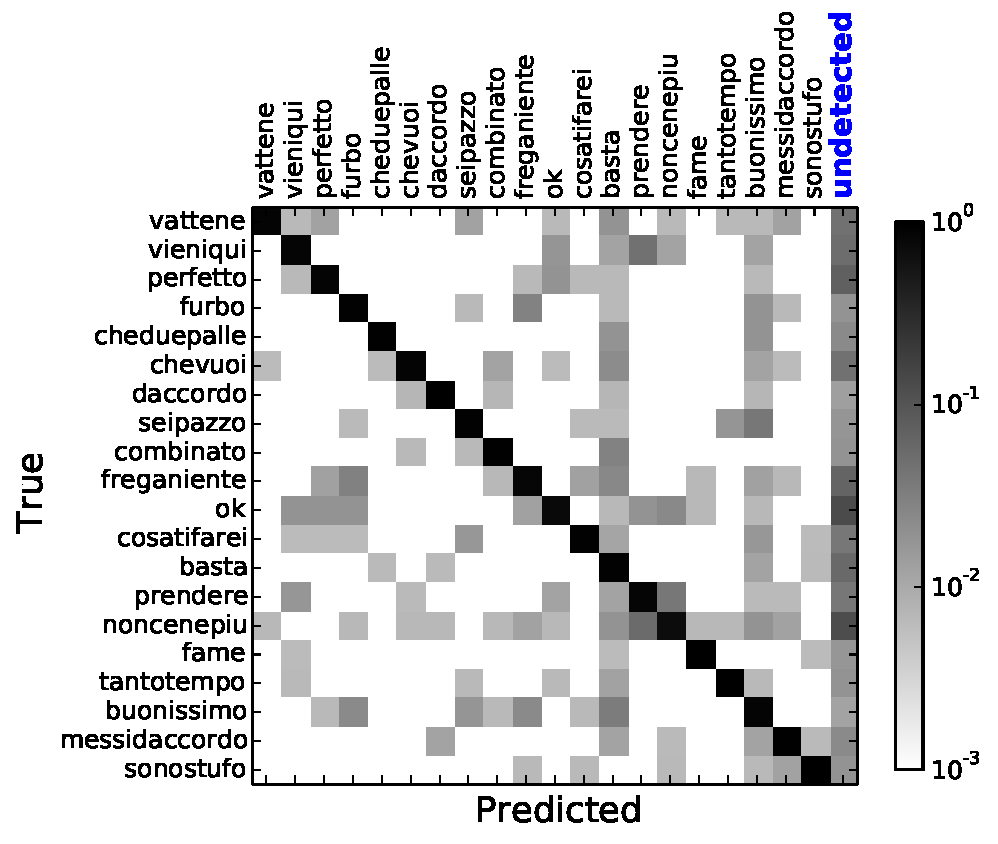
\includegraphics[width=\textwidth]{images/cm/cm_sk}
                \caption{Skeletal input prediction result.}
                \label{sk_cm}
        \end{subfigure}%
        ~ %add desired spacing between images, e. g. ~, \quad, \qquad, \hfill etc.
          %(or a blank line to force the subfigure onto a new line)

        \begin{subfigure}[c]{0.36\textwidth}
                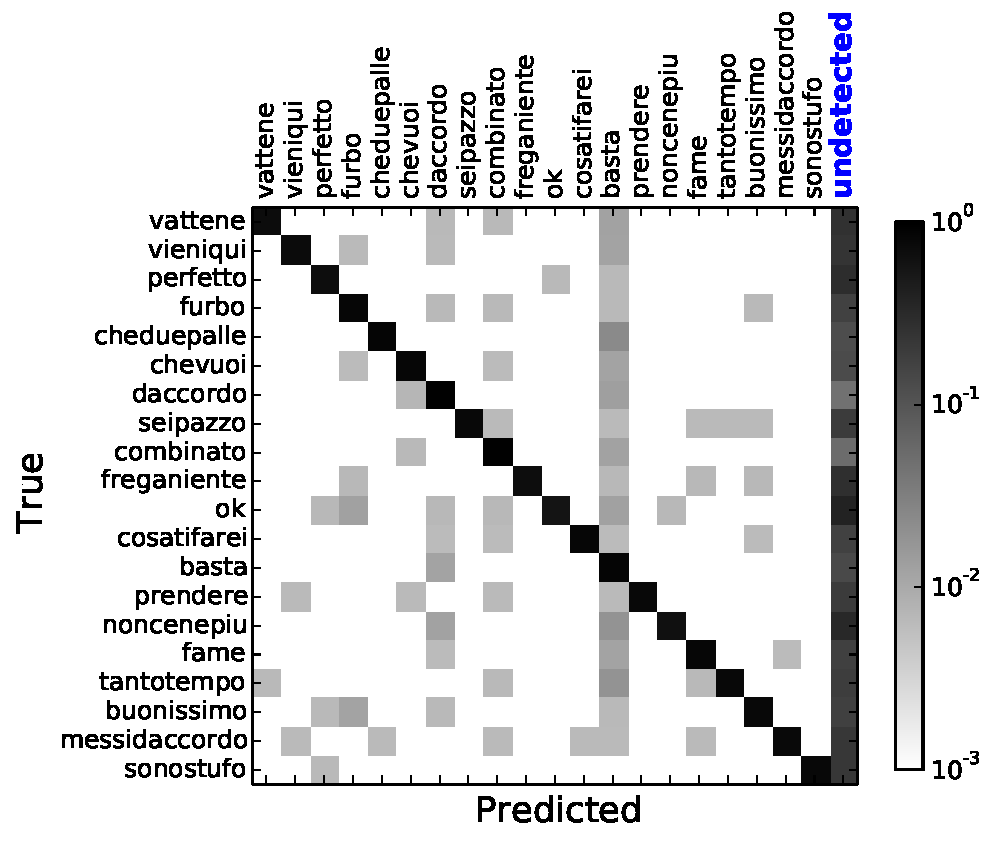
\includegraphics[width=\textwidth]{images/cm/cm_cnn}
                \caption{RGBD input prediction result.}
                \label{cnn_cm}
        \end{subfigure}

        ~ %add desired spacing between images, e. g. ~, \quad, \qquad, \hfill etc.
          %(or a blank line to force the subfigure onto a new line)
        \begin{subfigure}[c]{0.36\textwidth}
                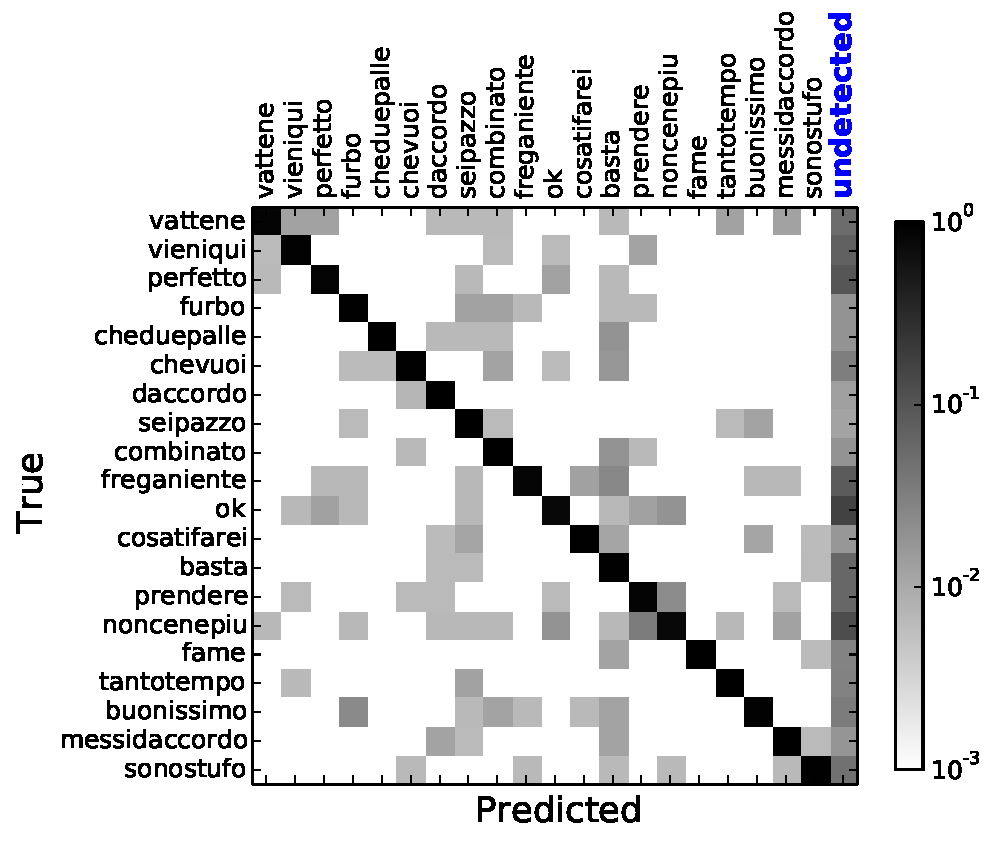
\includegraphics[width=\textwidth]{images/cm/cm_combination}
                \caption{Multimodal fusion prediction result.}
                \label{fusion_cm}
        \end{subfigure}

  \caption{Confusion Matrix for the skeletal input, RGBD input and multimodal fusion result.
  % Generally, the skeleton module has higher classification rate.
  Some gestures, \emph{e.g.} ``OK" and ``Non ce ne piu" differ primarily in hand poses. Hence, they are easier to be differentiated using the RGBD module than the skeleton module.
  }\label{confusion_matrix}
\end{figure}
%%%%%%%%%%%%%%%%%%%%%%%%%%%%%%%%%%%%%%%%%%%%%%%%%%%%%%%%%%

\begin{figure}[t]
        \centering


        \begin{subfigure}[c]{.2\textwidth}
        \centering
                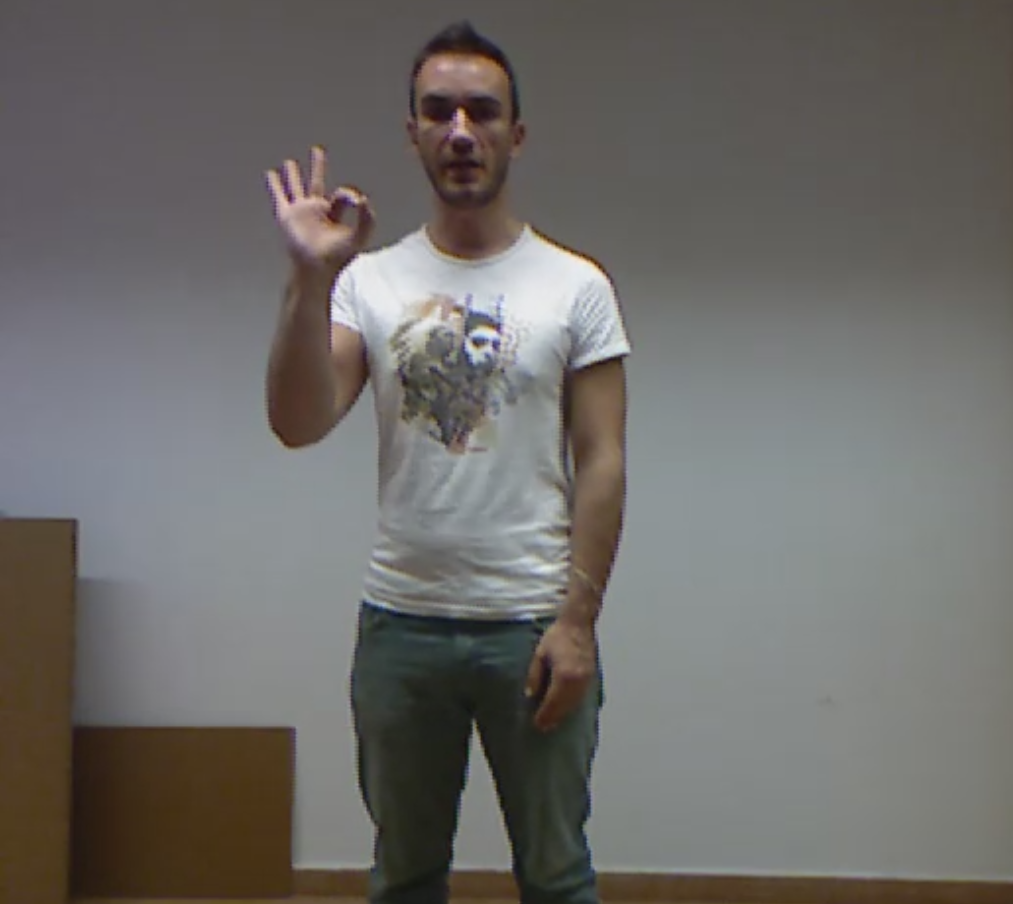
\includegraphics[width=3cm,height=3cm, trim=120 100 100 50, clip]{images/good}
                \caption{Well-recognised}
        \end{subfigure}%
        %
        \begin{subfigure}[c]{0.2\textwidth}
        \centering
                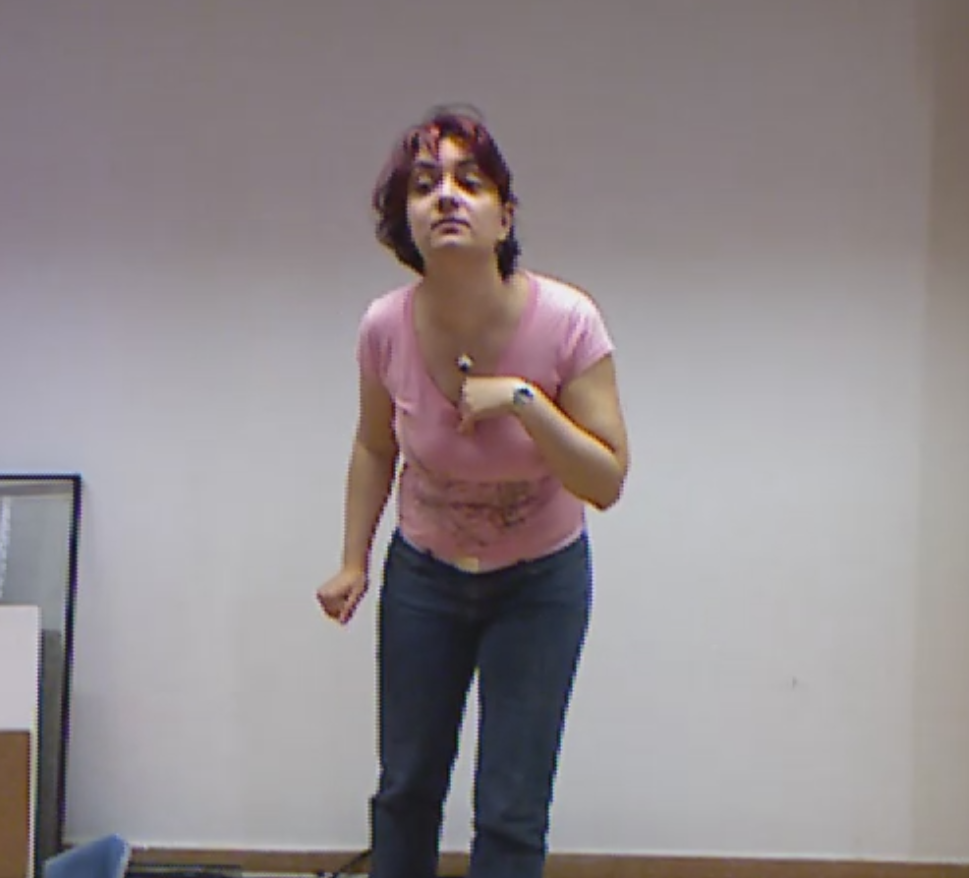
\includegraphics[width=3cm,height=3cm, trim=120 100 100 50, clip]{images/bad}
                \caption{Poorly-recognised}
        \end{subfigure}
  \caption{
  Examples of overall upper body movement's influence on system performance. Left (score: 0.94) performer almost kept static upper body whilst performing Italian sign language. Right (score: 0.34) performer moved vehemently when performing the gestures.
  }\label{good_bad_differ}
\end{figure}



\begin{figure}[t]
        \centering


        \begin{subfigure}[c]{.2\textwidth}
        \centering
                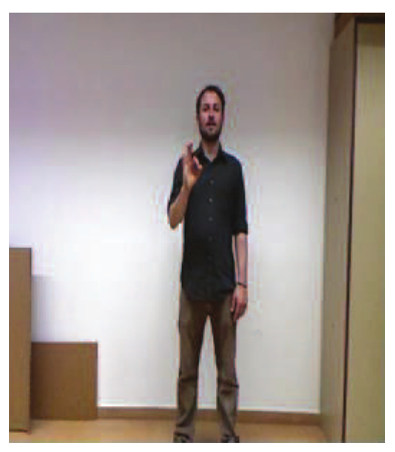
\includegraphics[width=2cm,height=3cm, trim=120 100 100 50, clip]{images/ok}
                \caption{``OK"}
        \end{subfigure}%
        %
        \begin{subfigure}[c]{0.2\textwidth}
        \centering
                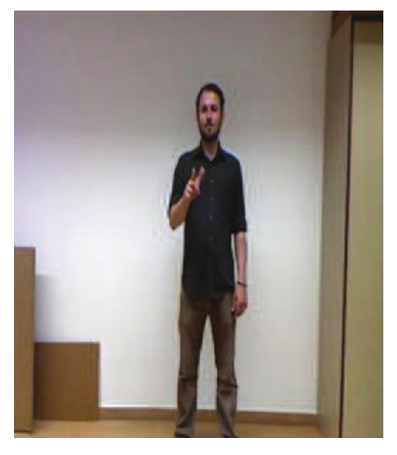
\includegraphics[width=2cm,height=3cm, trim=120 100 100 50, clip]{images/noncenepiu}
                \caption{``Non ce ne piu"}
        \end{subfigure}
  \caption{Examples of gestures that differ primarily in hand pose but not the arm motions.
  }\label{hand_differ}
\end{figure}

%%%%%%%%%%%%%%%%%%%%%%%%%%%%%%%%%%%%%%%%%%%%%%%%%%%%%%%%%%%%
 \begin{table}[t]
   \centering
        \begin{tabular}{|l||*{3}{c|}}\hline
            {Module}
            &\makebox[3em]{Skeleton}&\makebox[6em]{RGBD}&\makebox[3em]{Fusion}
            \\\hline\hline
            {~\cite{neverova2014multi}} Deep Learning (Step 4)                  &   0.7891     &  0.7990      & \textbf{0.8449}\\\hline
            {~\cite{neverova2014multi}} Deep Learning (multiscal)               &   0.8080     &  0.8096      & \textbf{ 0.8488}\\\hline
            {~\cite{Monnier2014multi}} 3 Set Skeletal \& HOG                   &   0.791     & -           & 0.8220 \\\hline
            {~\cite{Chang2014multi}}   Handcrafted features                       &  \textbf{0.7948}     & -           & 0.8268\\\hline
            {~\cite{Peng2014multi}}    Dense Trajectory                         &  -          & \textbf{0.7919}      & -\\\hline
            {~\cite{lio2014deep}}      CNN                                      &  -          & 0.7888      & -\\\hline
            {~\cite{wu2014deep}}    Deep Learning                               &  0.7468     & 0.6371      & 0.8045\\\hline \hline
            \textbf{\emph{DDNN}} (this work)                                    &  0.7792    & 0.7168  & 0.8091\\\hline
        \end{tabular}
    \caption{
    Comparison of results in terms of Jaccard index between different network structures and various modules.
          }
          \label{Table_baseline}
\end{table}


\subsection{Computational Complexity}
\label{sec:ComputationalComplexity}

Although training the deep neural network using stochastic gradient descent is computationally intensive, once the model finishes training, our framework can perform real-time video sequence labelling with a low inference cost.
Specifically, a single feed forward neural network incurs linear computational time ($\mathcal{O}(T)$) and is efficient because it requires only matrix products and convolution operations. The complexity of the Viterbi algorithm is $\mathcal{O} (T* |S|^2)$ with $T$ the number of frames and $|S|$ the number of states.

Using a modern GPU (GeForece GTX TITAN Black), our multimodal neural network can be deployed at 90 FPS using Theano library~\cite{Bastien-Theano-2012} which is 6 times of real time (15 FPS). The preprocessing part takes most of the time and our un-optimized preprocessing pipeline is 25 FPS and Viterbi decoding is 90 FPS. Hence, the overall system can achieve faster than real-time performance.





\endinput
